\documentclass[journal]{IEEEtran}

% Packages
\usepackage{graphicx}
\usepackage{amsmath}
\usepackage{cite}
\usepackage{caption}
\captionsetup[table]{name=}

% Title
\title{Lab 2: Understanding of the low-level characteristics of the visual information: colors and color spaces}
\author{Bruno Luiz Dias Alves de Castro \\ Victor Gabriel Mendes Sündermann}
\date{\today}

\begin{document}

\maketitle

\begin{abstract}
During this lab, we will develop a Python application with support of the library OpenCV to identify skin in Images. Throughout the execution of multiple tests with different lighting and color schemes, we observe the nunaces of each different color spaces, and how different lighting conditions can affect the outcome.
\end{abstract}

\section{Introduction}
As it happens with every digital representation of the real world in the digital domain, images do not have an one to one equivalence in our computers. By definition, images are continuous signals, and such things don't have a direct representation in our binary structures.

In order to represent images in our computers, we need to discretize them. This means that we need to sample the image in a grid, and then quantize the values of each pixel. This process is called digitization, and comees with a few drawbacks. The most important one is that we lose information in the process. This means that we can't recover the original image from the digital representation.

One other import aspect of this representation, is the need to choose a color space to work with. A color space is a mathematical model that allows us to represent colors in a way that is easy to manipulate. The most common color space is the RGB color space, which is the one used in most digital devices. However, there are other color spaces that are more suitable for image processing, such as the RGB and HSV color spaces.

In this lab, we will explore two color spaces, the HSV and the YCbCr color spaces, and try to use them to segment images in different lighting conditions.

\section{Color Spaces}

As explained in the introduction, a color space is a mathematical model that allows us to represent colors in a way that is easy to manipulate. The most common color space is the RGB color space, which is the one used in most digital devices. In the sections, we will explore the two target color spaces of this lab, the HSV and the YCbCr color spaces.

\subsection{RGB Color Space}

The RGB color space is the most common color space in digital devices. It is an additive color space, that is, the colors are represented by adding different amounts of red, green and blue. This color space is very intuitive, since it is based on the way our own eyes perceive color.

In this space, each pixel is represented by three bytes, one for each color component. The values of each color range from 0 to 255, which means that there are 256 possible values for each color. This means that there are $256^3 = 16777216$ possible colors in this color space.

\subsection{HSV Color Space}

The HSV color space is a cylindrical color space, which means that it is represented by a cylinder. The HSV color space is based on the RGB color space. The HSV color space is composed of three components, the Hue, the Saturation and the Value. The Hue component represents the color itself, and is represented by an angle in the cylinder. The Saturation component represents the purity of the color, and is represented by the distance from the center of the cylinder. The Value component represents the brightness of the color, and is represented by the height of the cylinder.

In this space, each pixel is represented by three bytes, one for each component. The values of the Hue component range from 0 to 179, the values of the Saturation component range from 0 to 255, and the values of the Value component range from 0 to 255. This means that there are $180 \times 256 \times 256 = 11796480$ possible colors in this color space.

\subsection{YCbCr Color Space}

The YCbCr color space is a color space that is based on the RGB color space. It is a subtractive color space, which means that the colors are represented by subtracting different amounts of cyan, magenta and yellow. The YCbCr color space is also device dependent, which means that the same color can be represented differently in different devices. The YCbCr color space is composed of three components, the Luminance, the Blue Chrominance and the Red Chrominance. The Luminance component represents the brightness of the color, and is represented by the Y component. The Blue Chrominance component represents the blue color, and is represented by the Cb component. The Red Chrominance component represents the red color, and is represented by the Cr component.

In this space, each pixel is represented by three bytes, one for each component. The values of the Luminance component range from 0 to 255, the values of the Blue Chrominance component range from -128 to 127, and the values of the Red Chrominance component range from -128 to 127. This means that there are $256 \times 256 \times 256 = 16777216$ possible colors in this color space.

\section{Methodology}

In this section, we will describe the methodology used in this lab. We will describe the tools used, the experiments performed, and the results obtained.

\subsection{Tools}

During this lab, we used three main technologies. The Python programming language (through the Jupyter Notebook), the OpenCV library, and the GIMP graphics editor, to create our ground truth images.

\subsection{Image Acquisition and Ground Truth}

To perform our experiments, we acquired three different hand images, each one in different lighting conditions. The first used a yellow light, the second a white light, and the third a combination of both.

For the ground truth, we simply separated the background from the hand using GIMP

\subsection{Experiments}
In order to ajust the parameters, we altered by hand the values of the parameters, and then observed the results. They were adjusted to achive the best results possible for the first image, and then the same parameters were used for the other images.

\begin{table}[htbp]
\centering
\begin{tabular}{ccc}
    \rotatebox{-90}{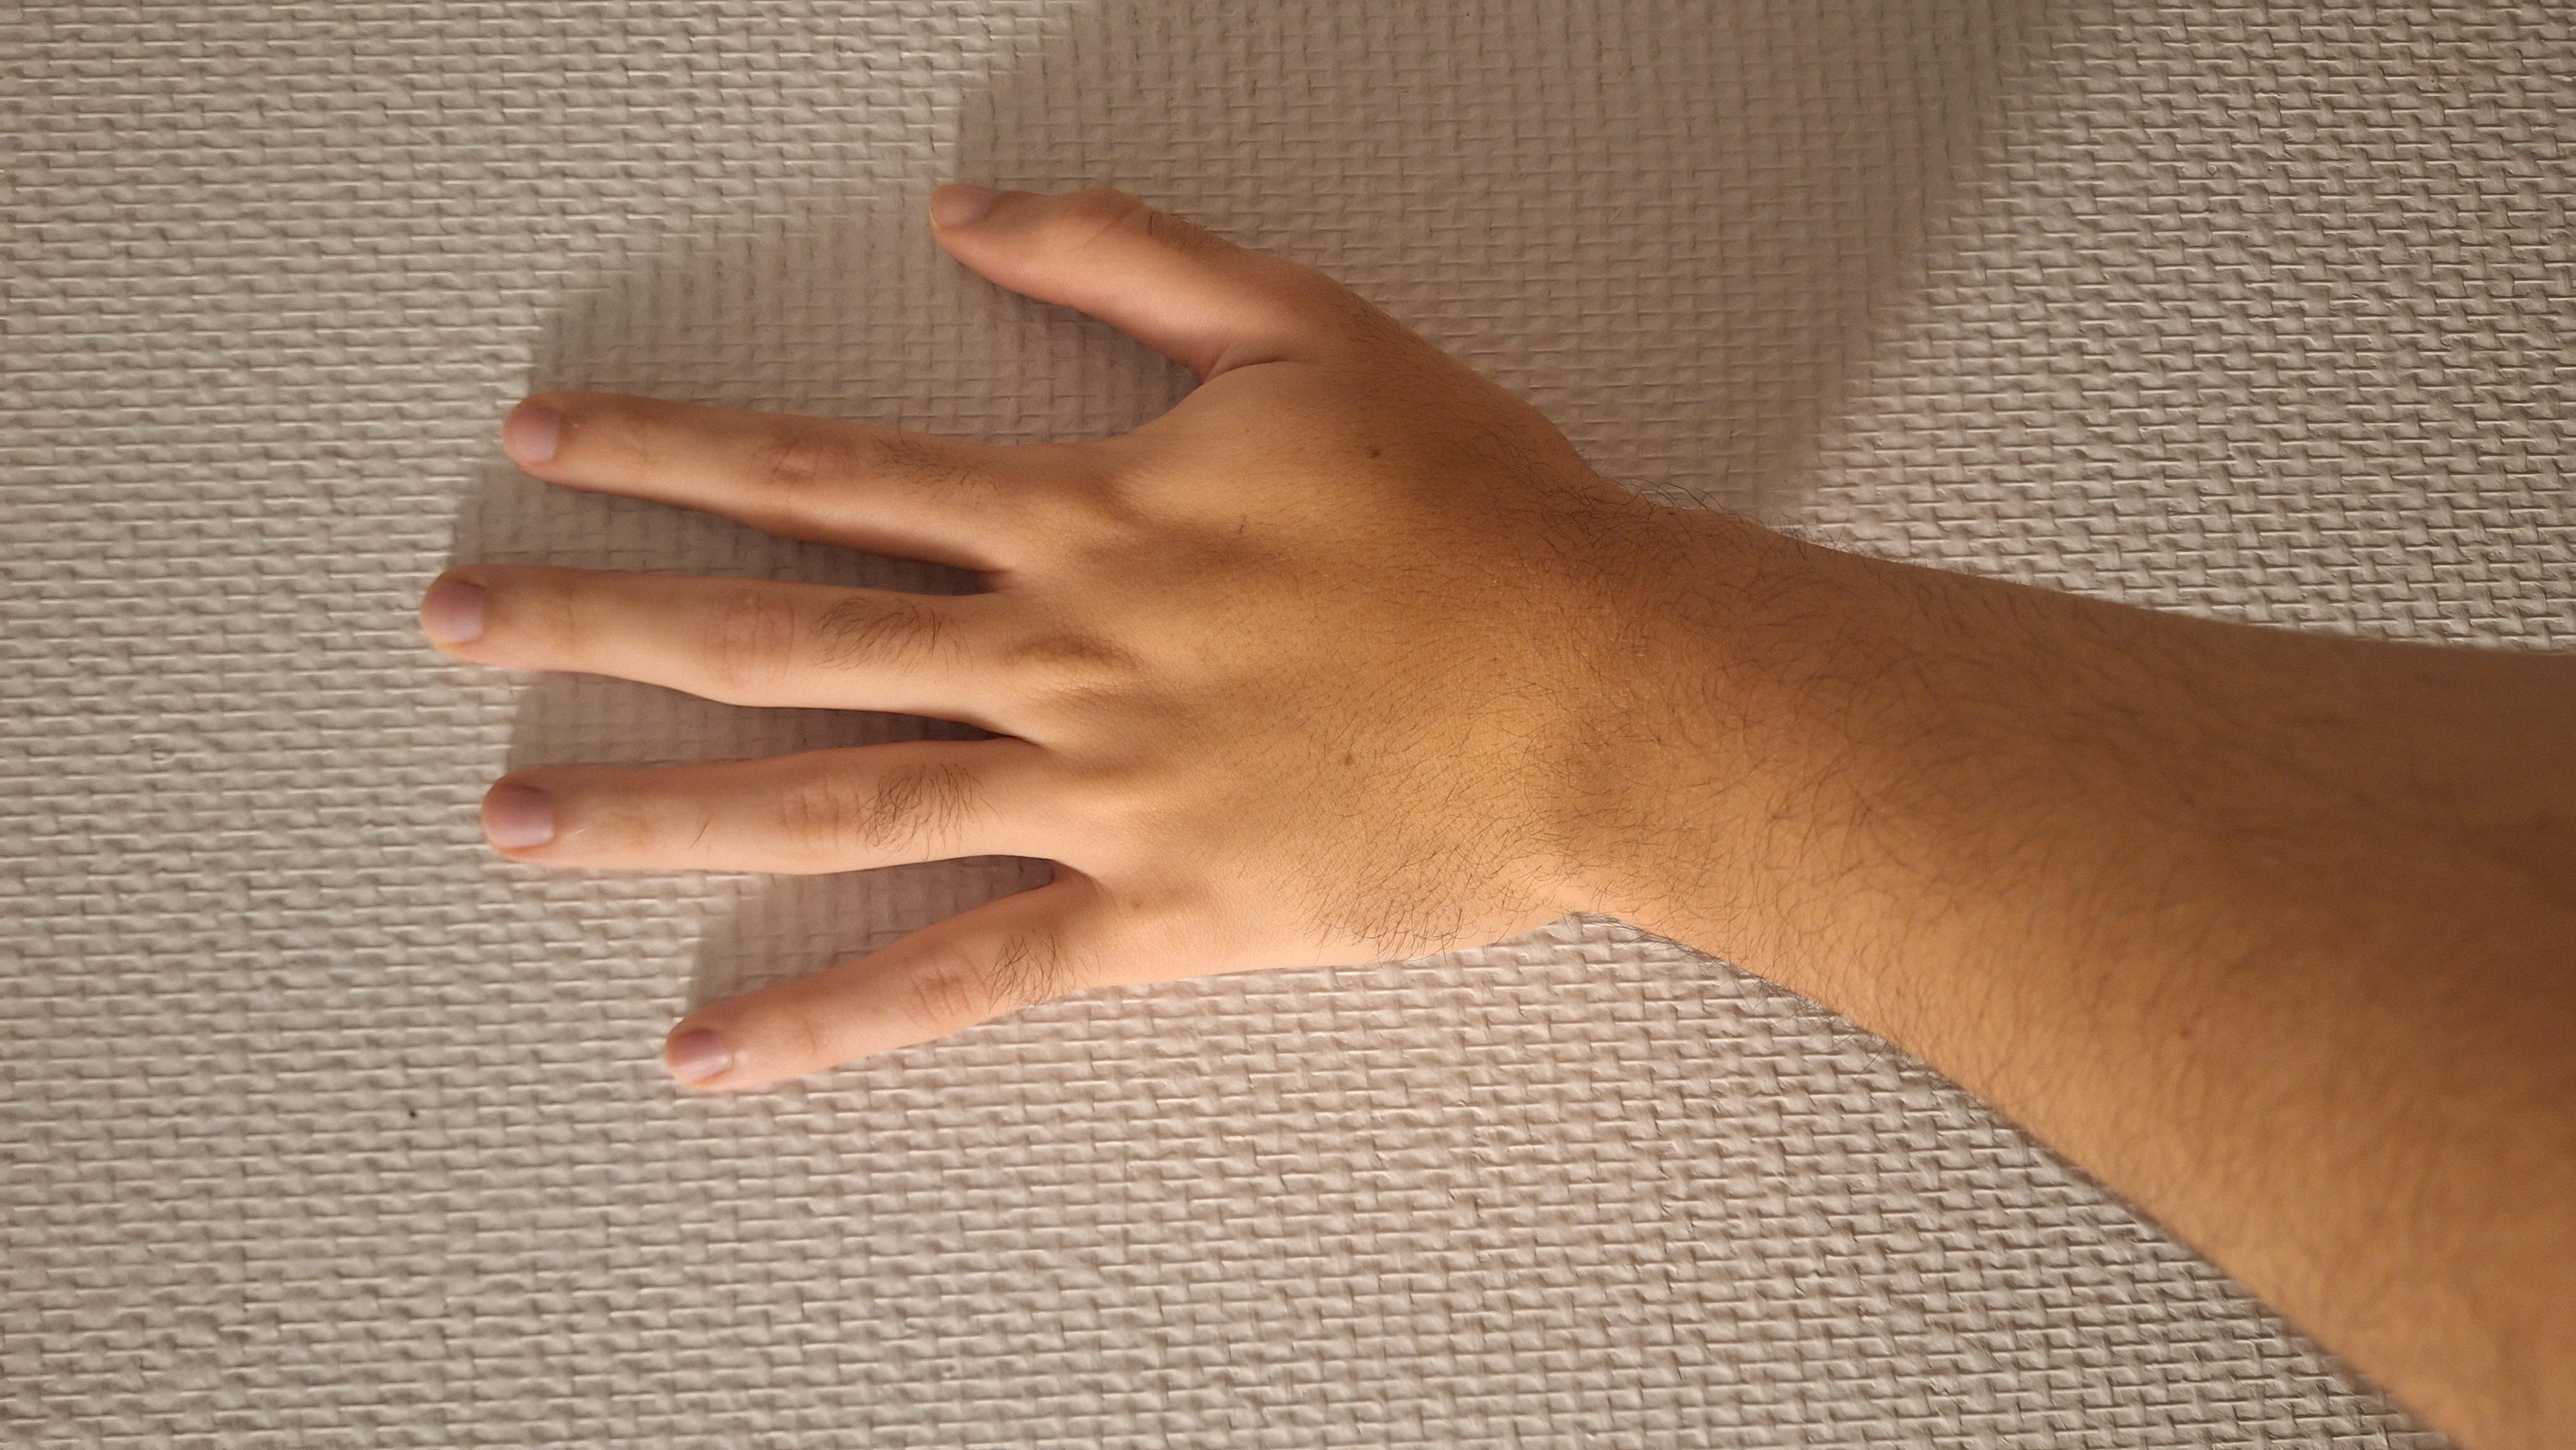
\includegraphics[width=0.4\linewidth]{../images/hand1.jpg}} & \rotatebox{-90}{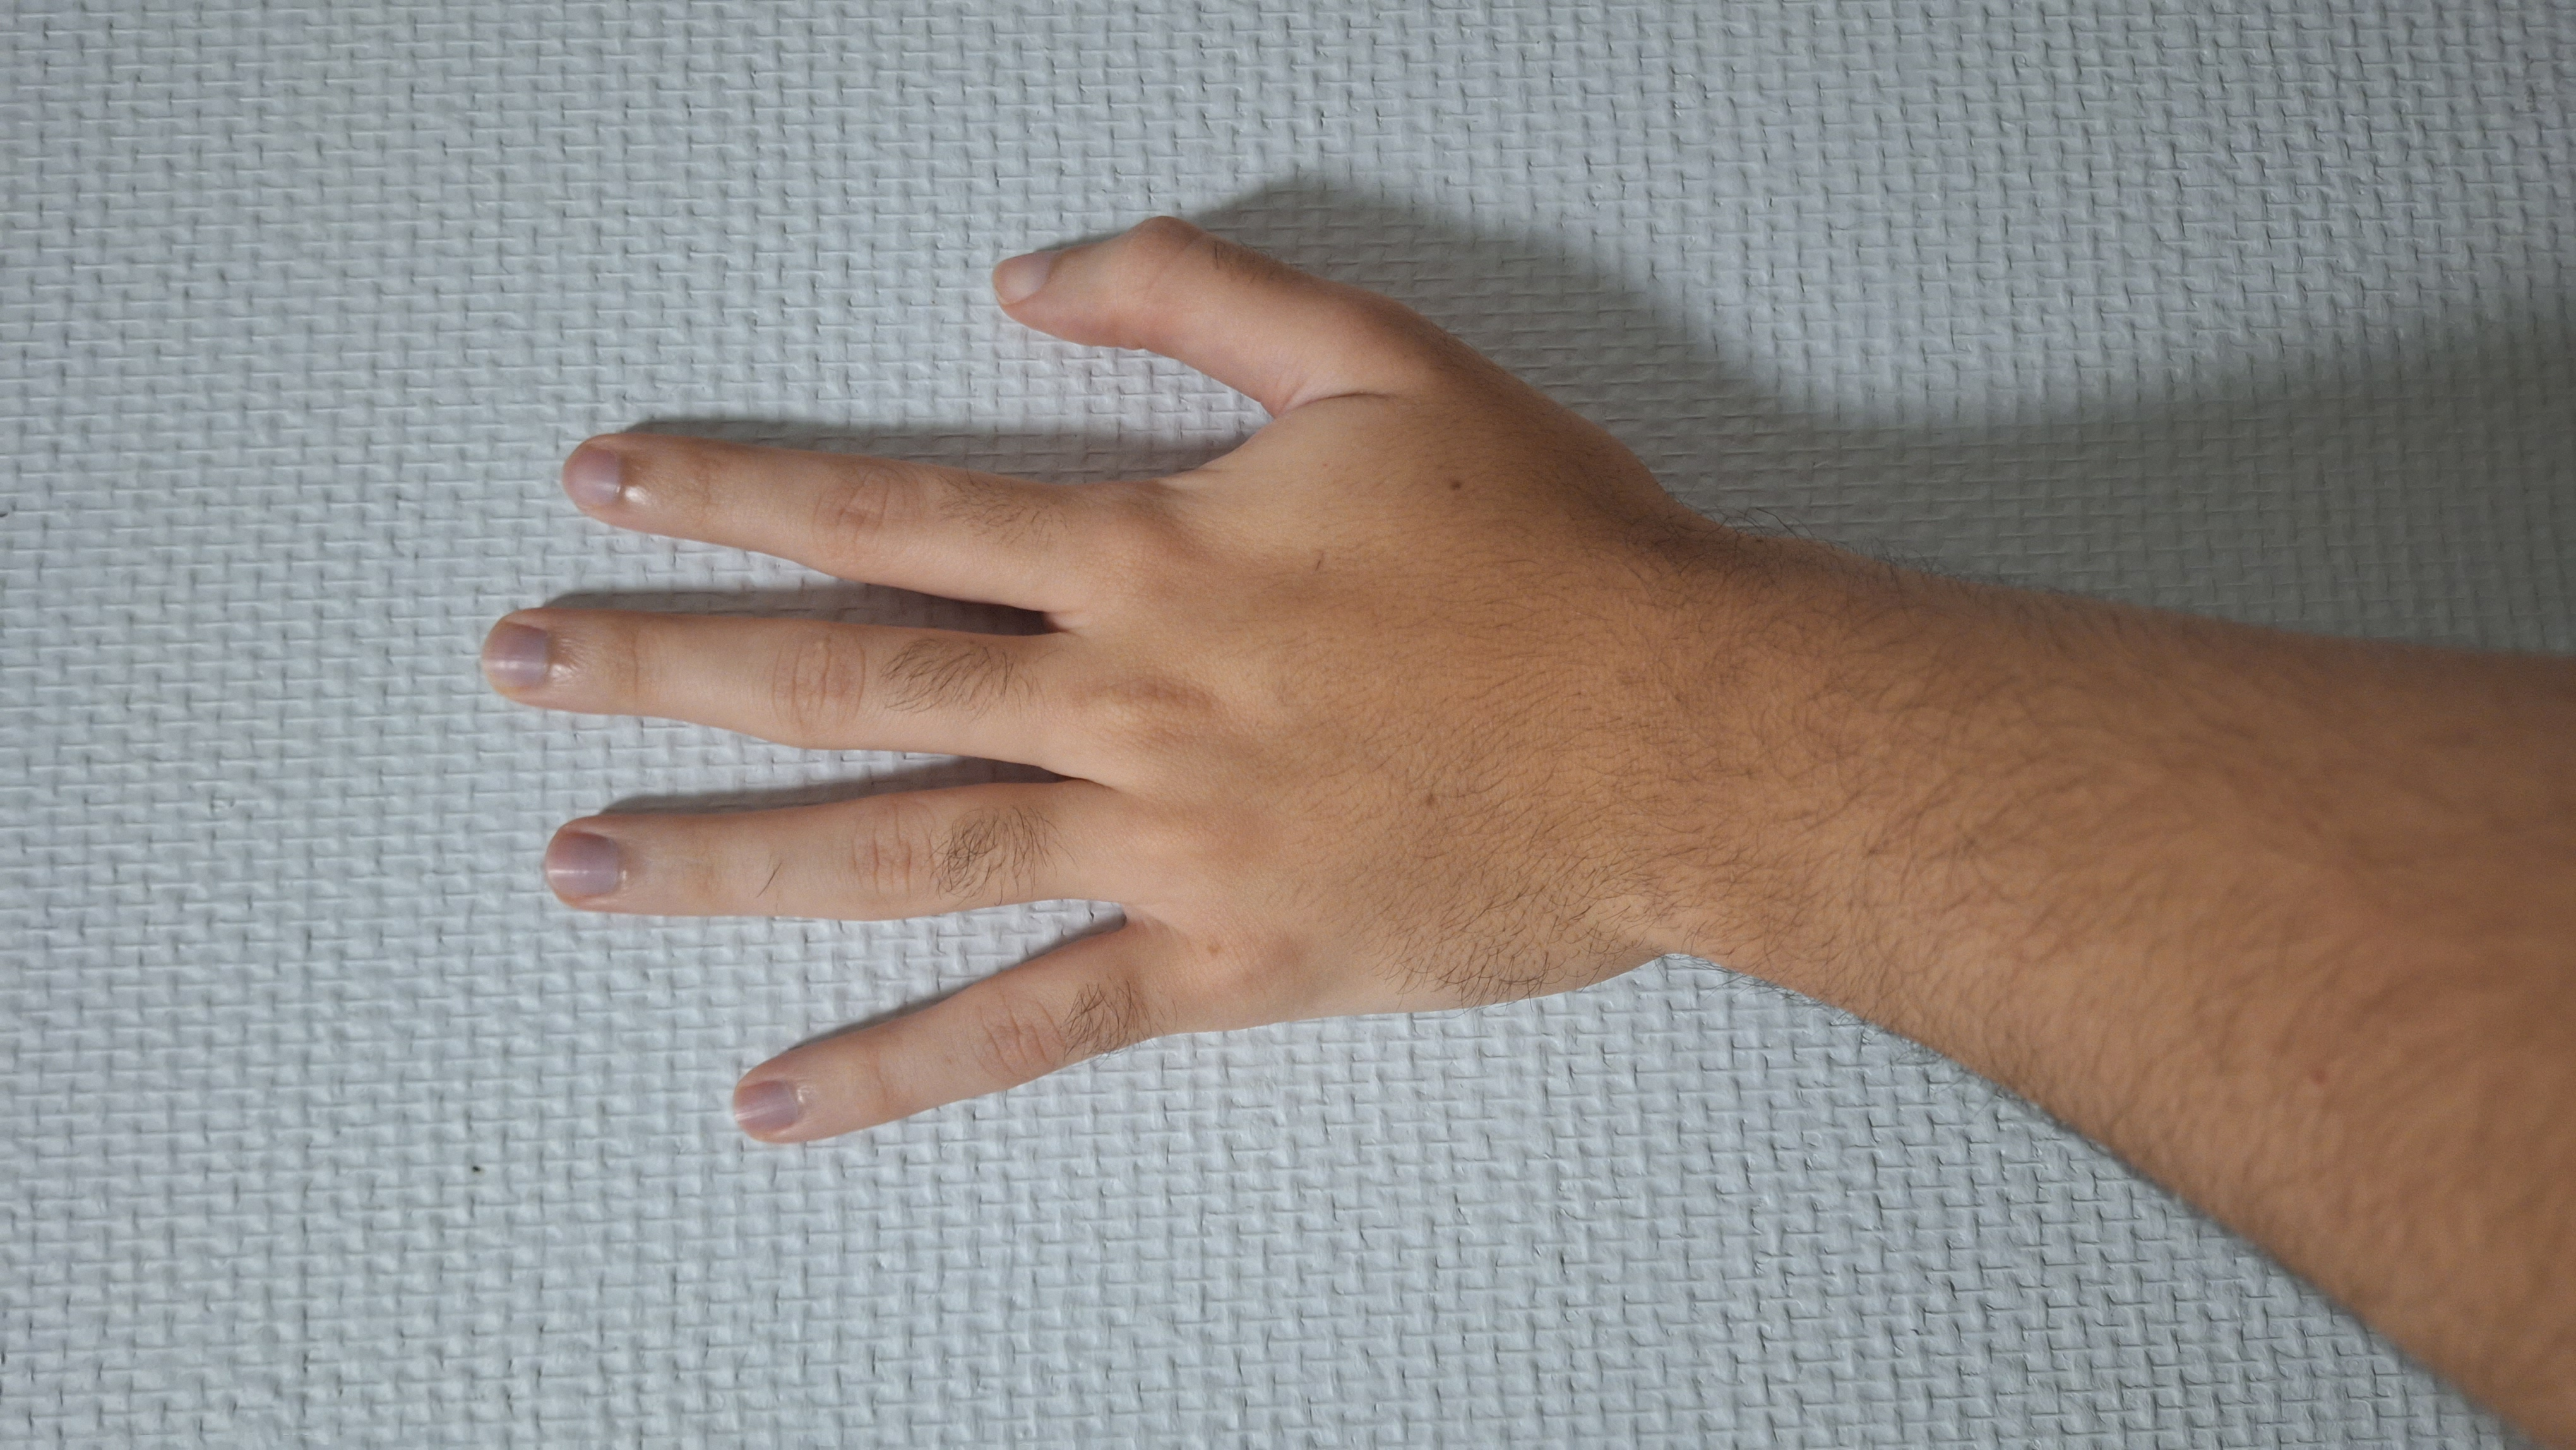
\includegraphics[width=0.4\linewidth]{../images/hand2.jpg}} & \rotatebox{-90}{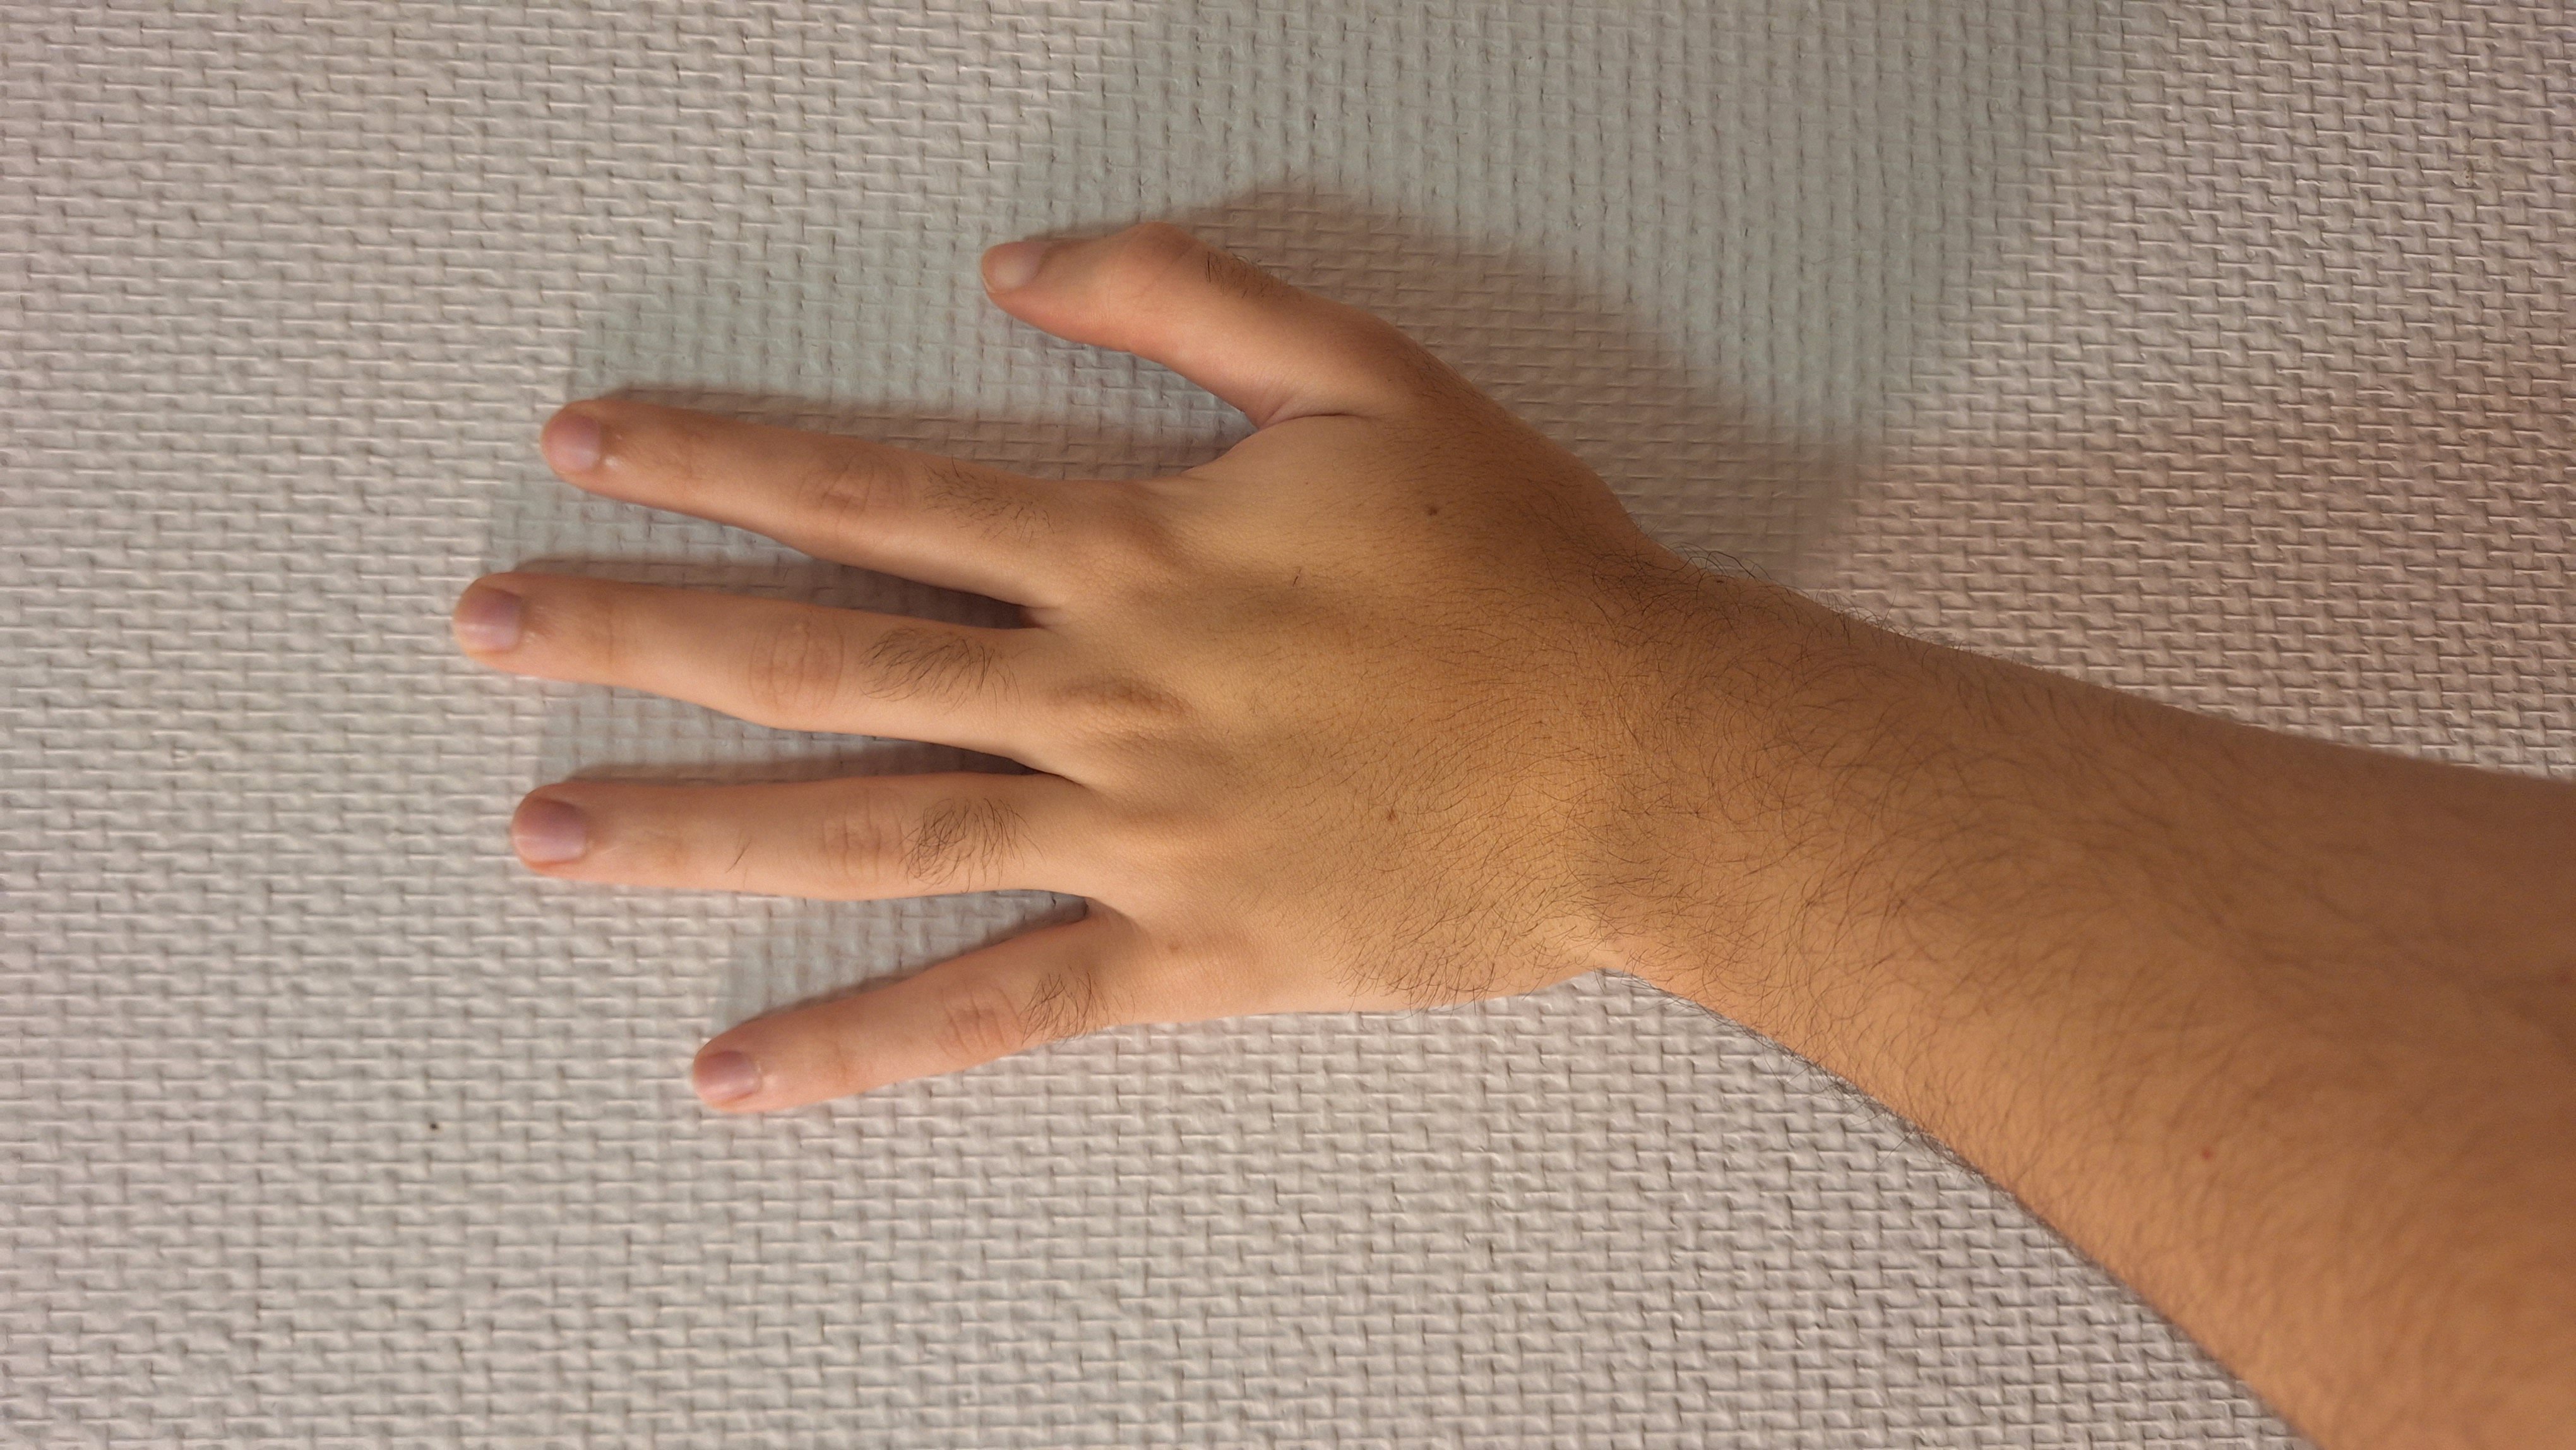
\includegraphics[width=0.4\linewidth]{../images/hand3.jpg}} \\
    \rotatebox{-90}{
\includegraphics[width=0.4\linewidth]{../images/hand1_GT.jpg}} & \rotatebox{-90}{
\includegraphics[width=0.4\linewidth]{../images/hand2_GT.jpg}} & \rotatebox{-90}{
\includegraphics[width=0.4\linewidth]{../images/hand3_GT.jpg}} \\
\end{tabular}
\caption{Original images and ground truth images.}
\label{tab:images}
\end{table}

\section{Results}

\begin{table}[!htbp]
\centering
\begin{tabular}{cc}
    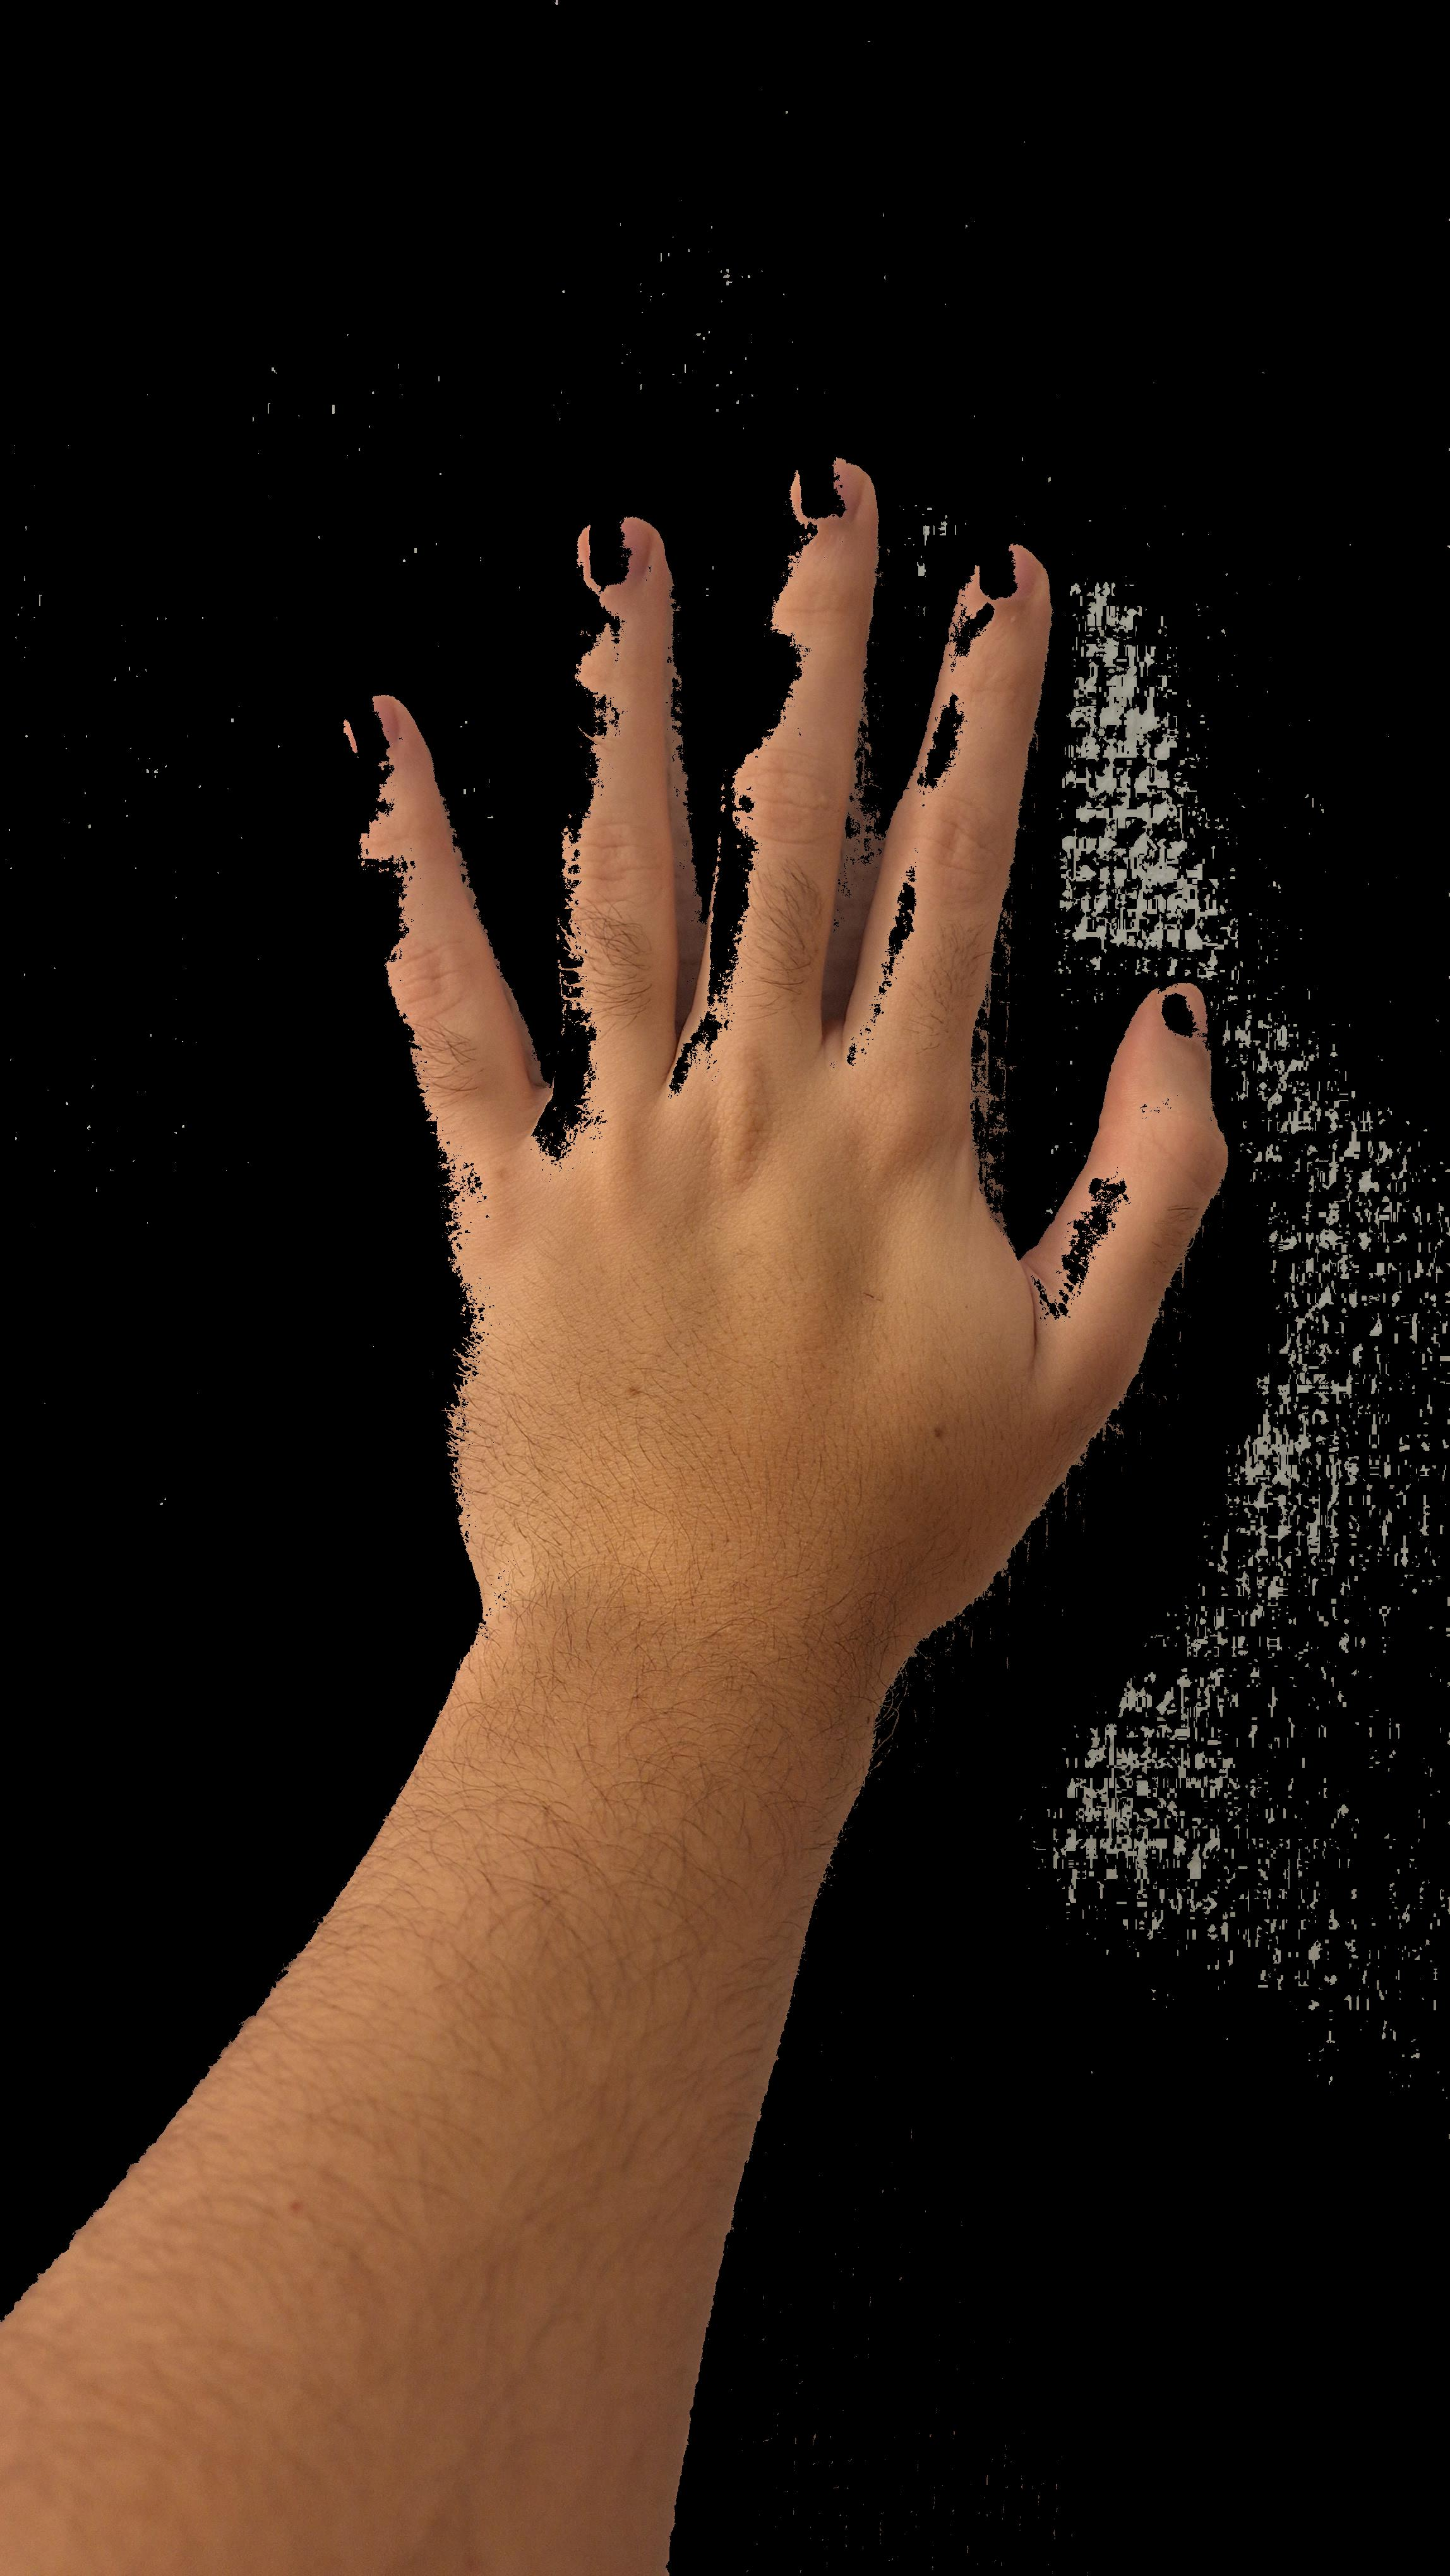
\includegraphics[width=0.3\linewidth]{../images/results/hand1_skin_hsv.jpg} & 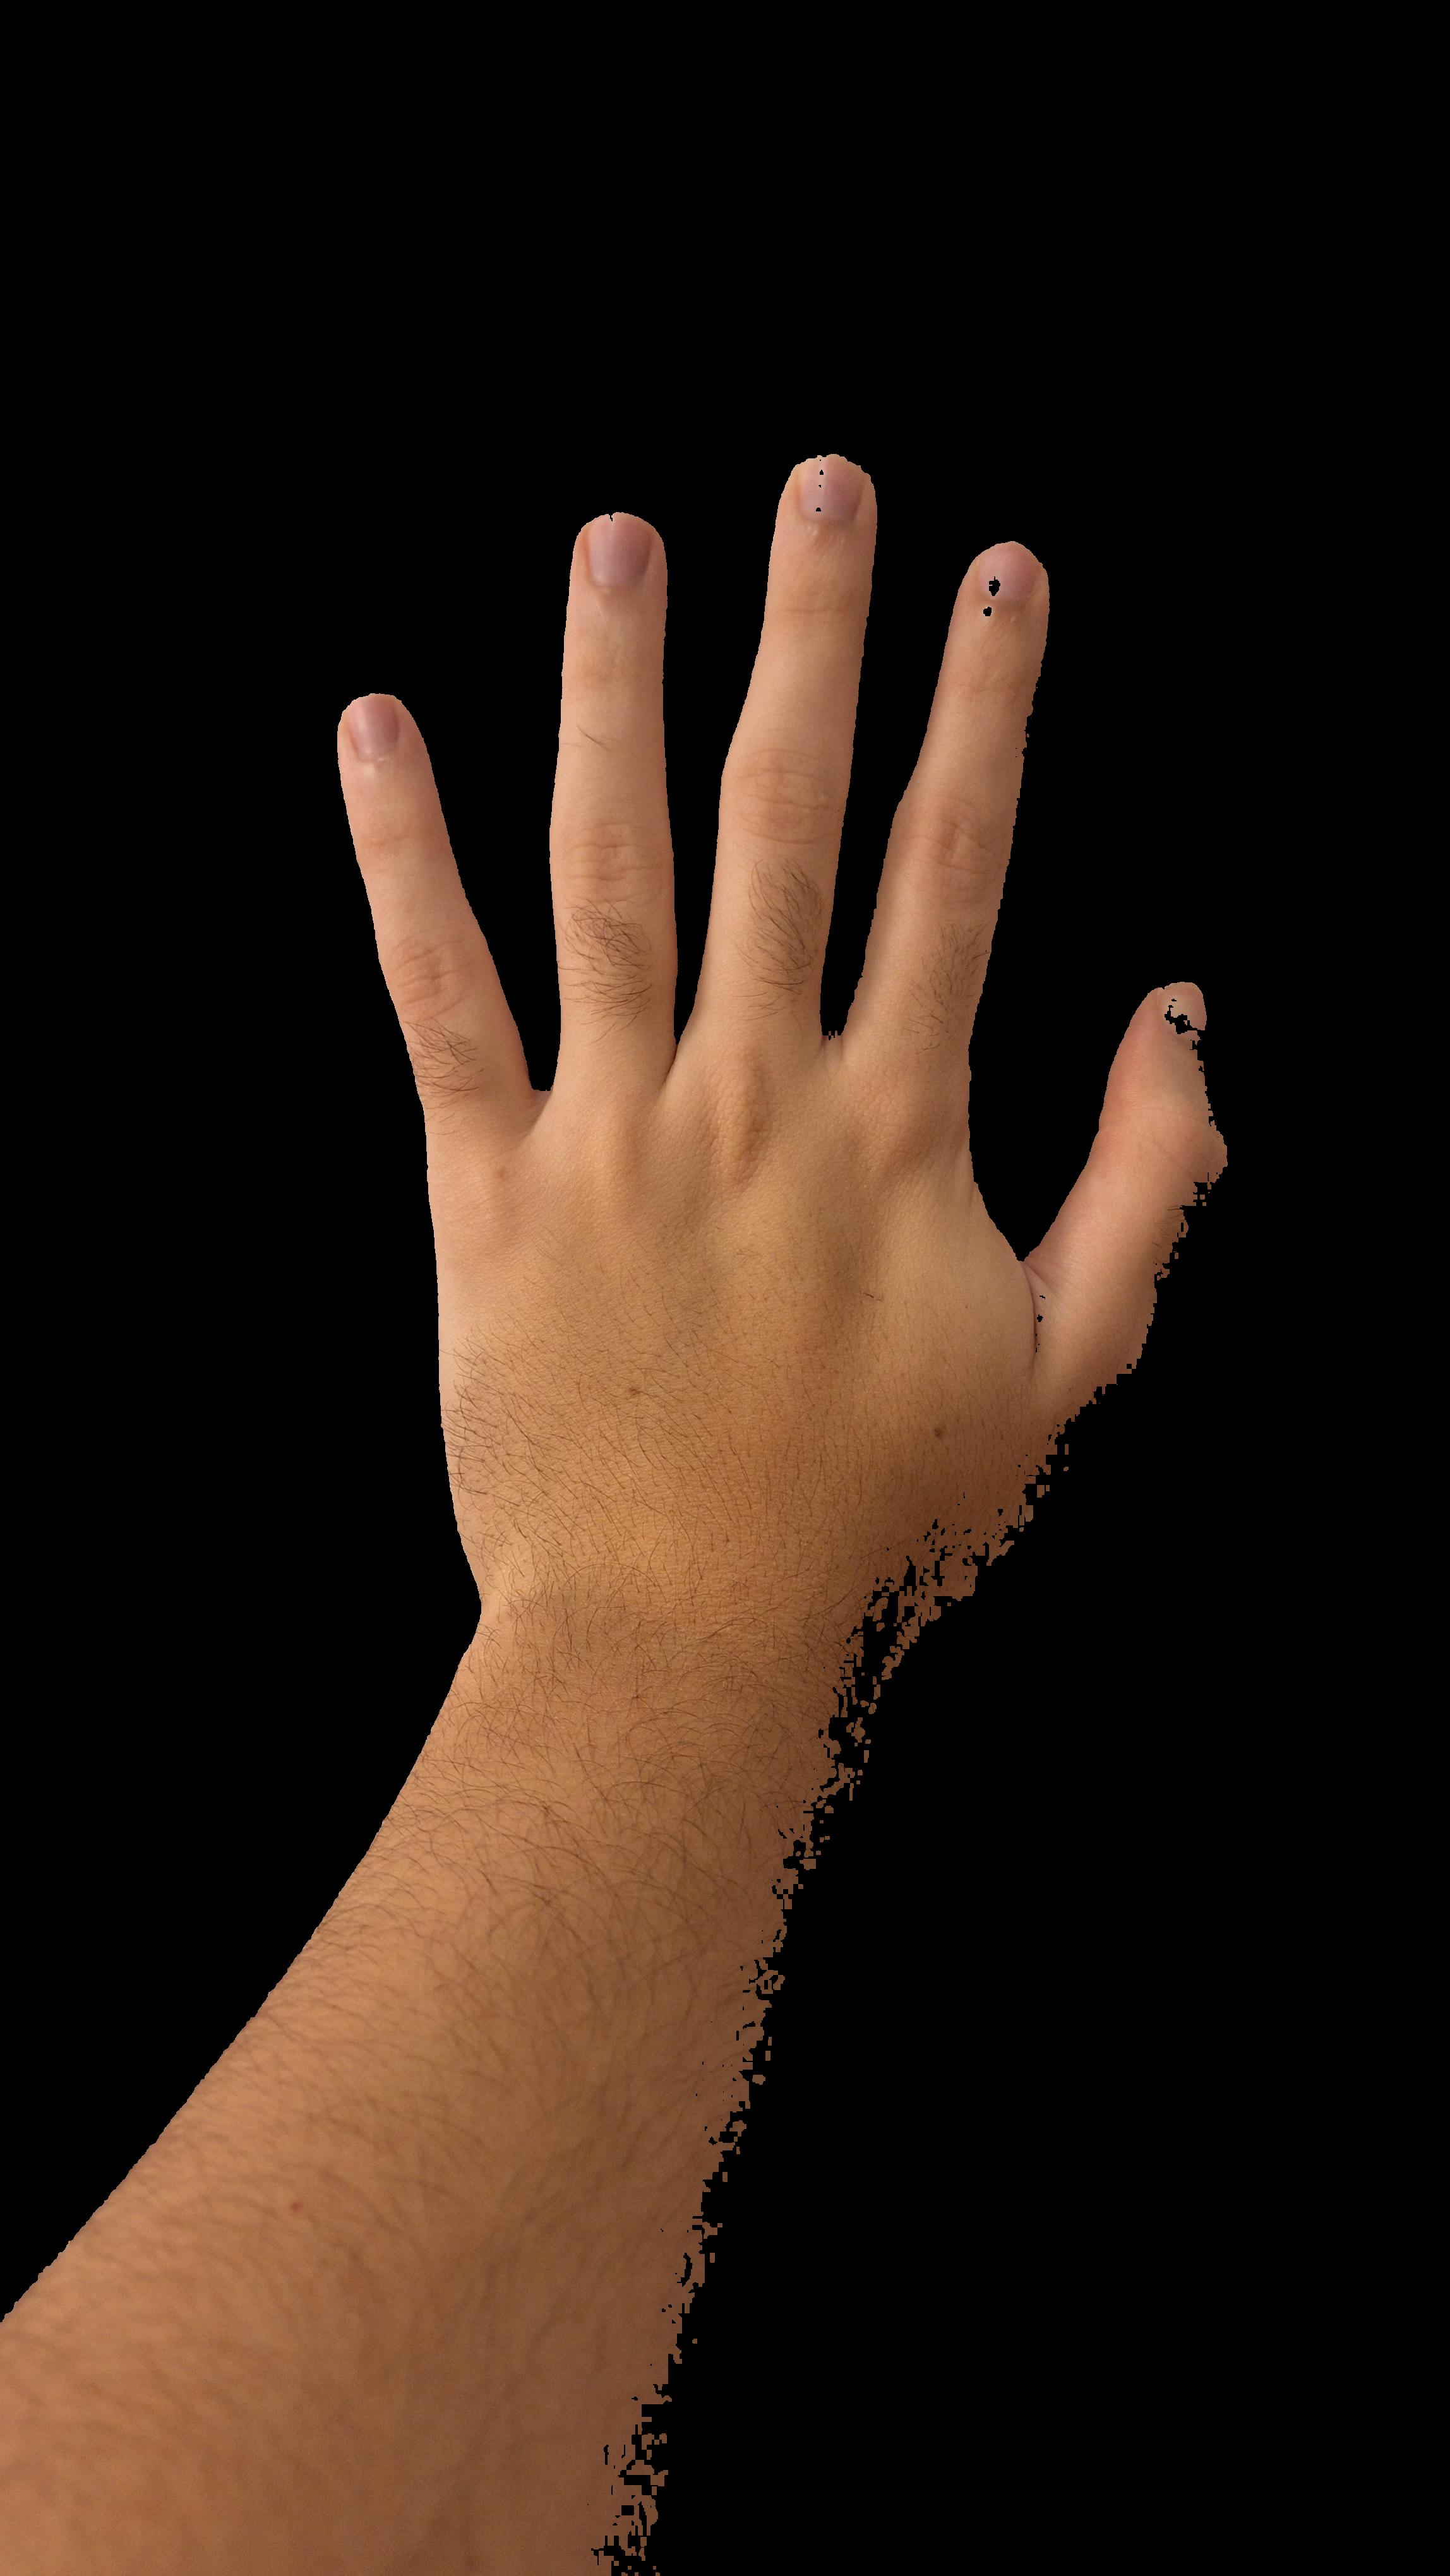
\includegraphics[width=0.3\linewidth]{../images/results/hand1_skin_ycc.jpg} \\
\end{tabular}
\caption{Image 1 results (HSV and YCbCr).}
\label{tab:imagens}
\end{table}

\begin{table}[!htbp]
\centering
\begin{tabular}{cc}
    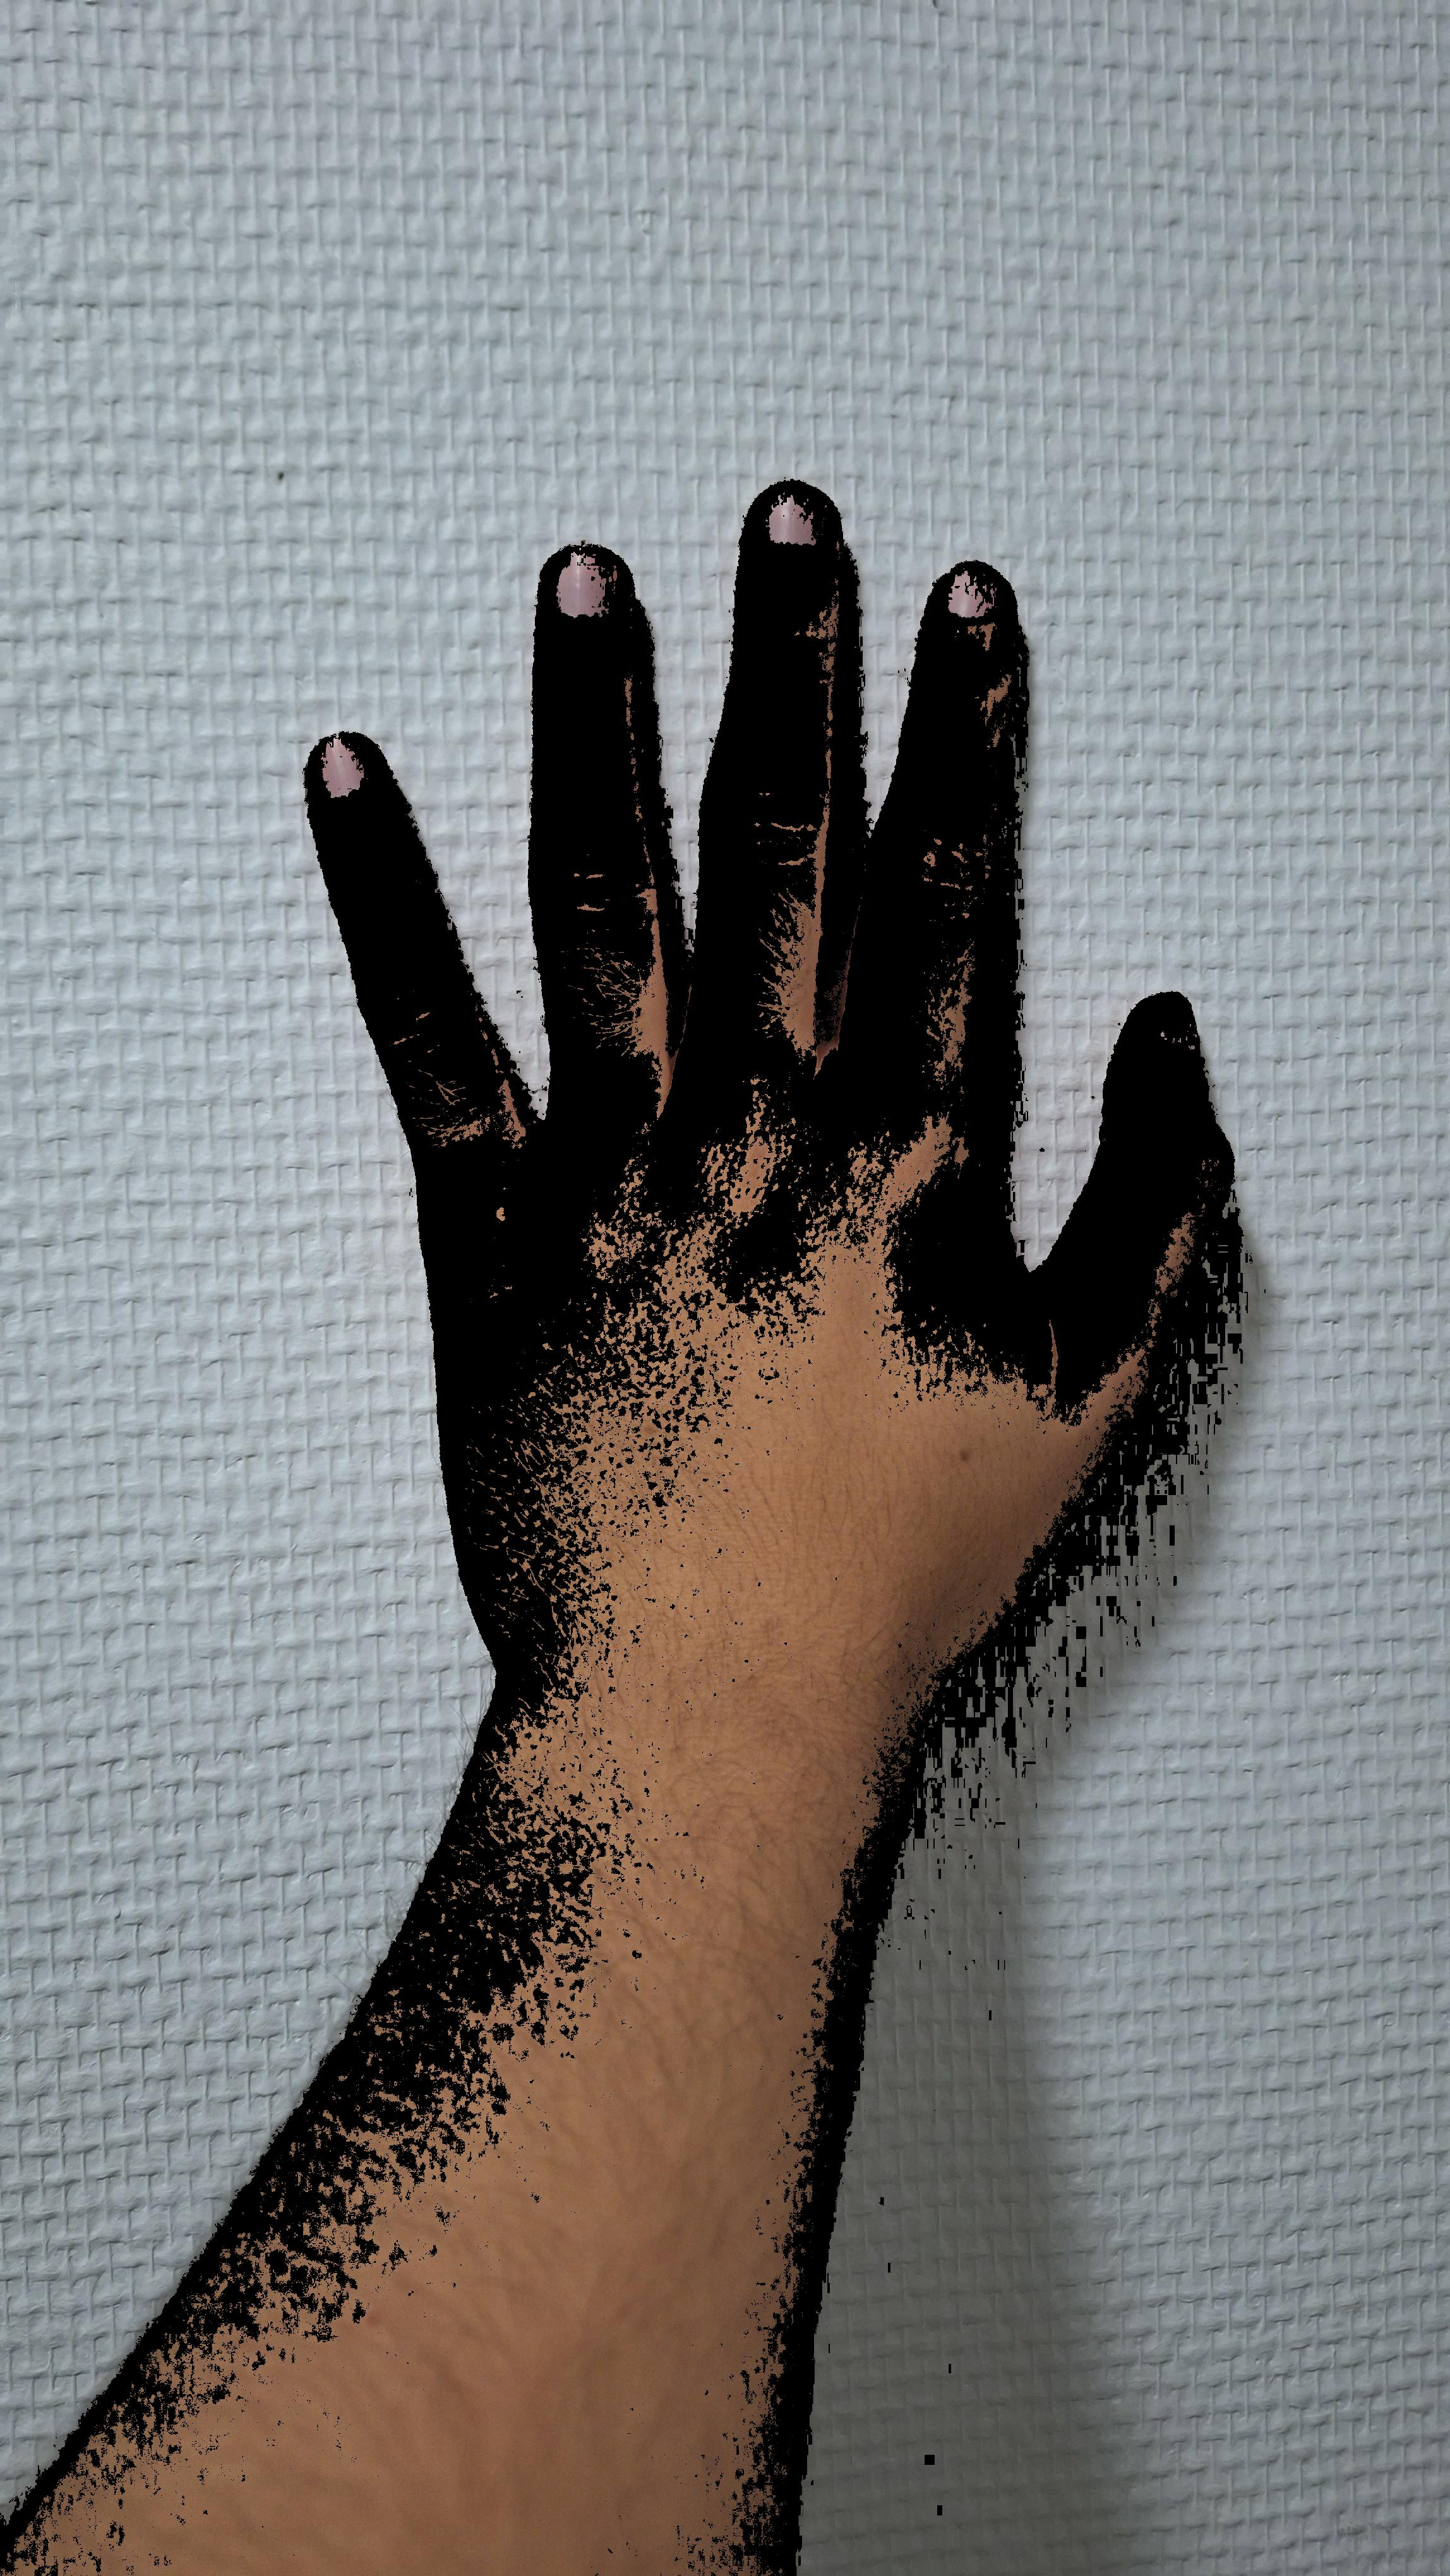
\includegraphics[width=0.3\linewidth]{../images/results/hand2_skin_hsv.jpg} & 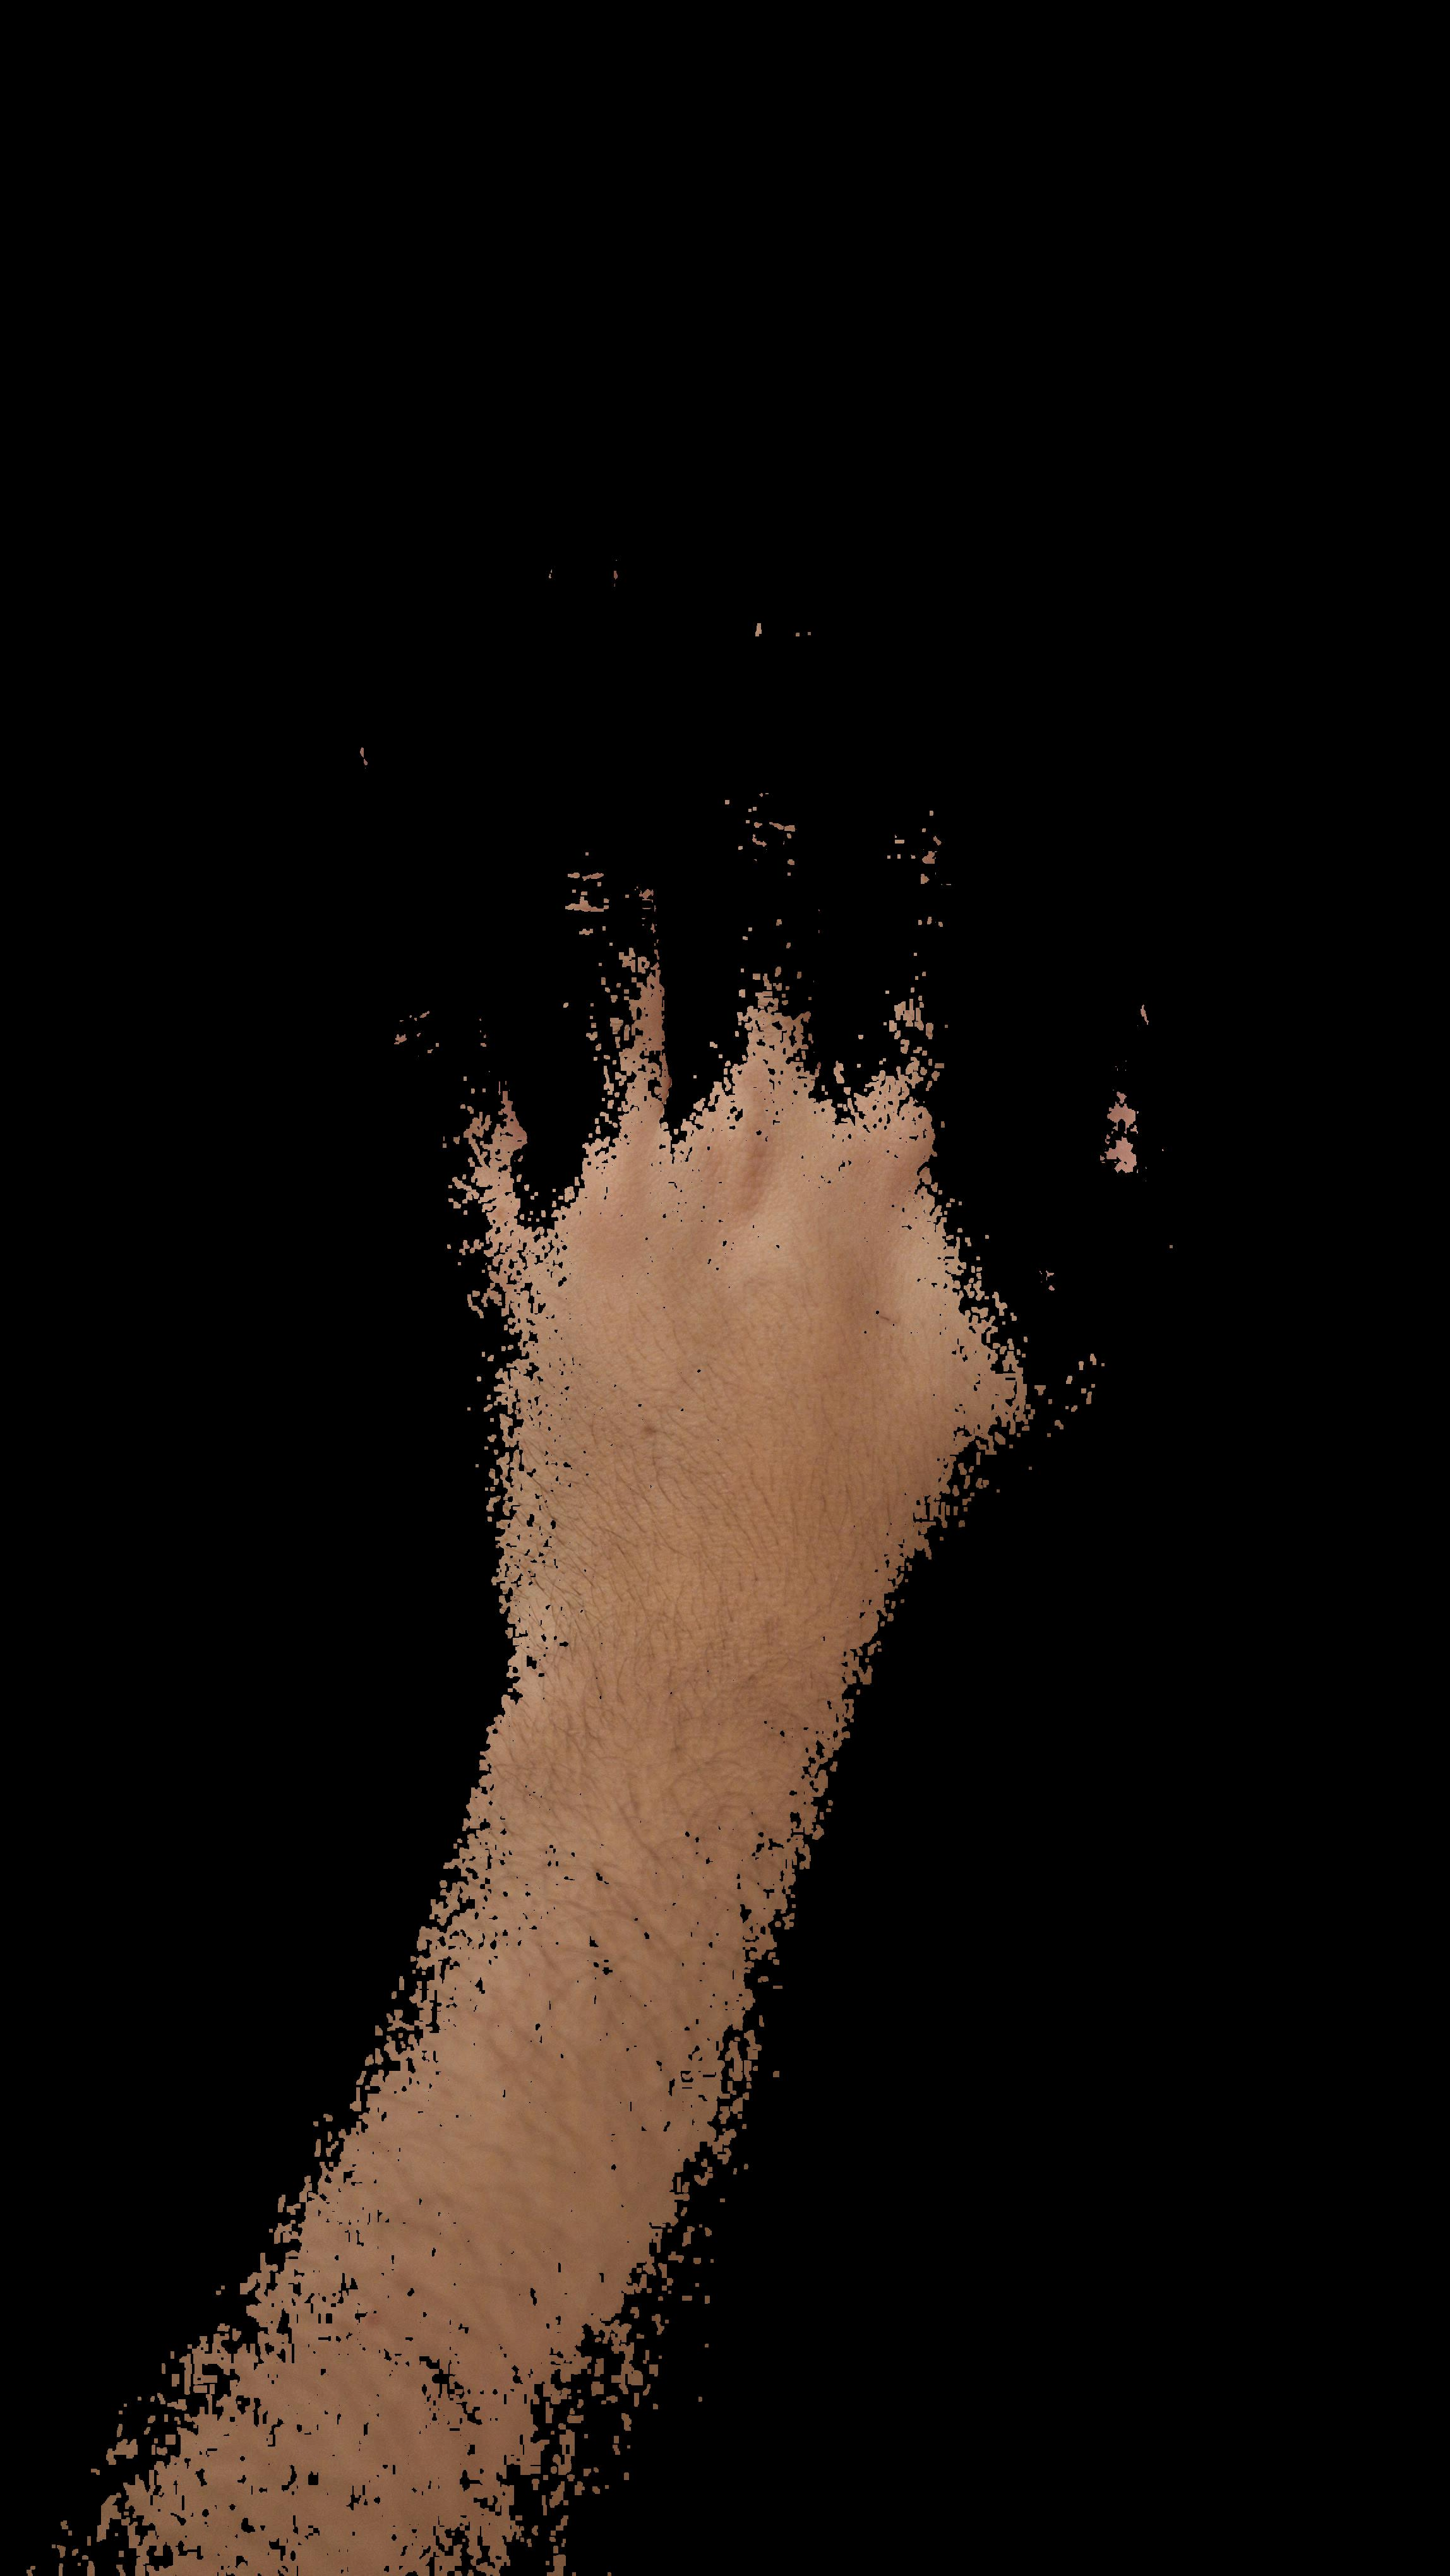
\includegraphics[width=0.3\linewidth]{../images/results/hand2_skin_ycc.jpg} \\
\end{tabular}
\caption{Image 2 results (HSV and YCbCr).}
\label{tab:images2}
\end{table}

\begin{table}[!htbp]
\centering
\begin{tabular}{cc}
    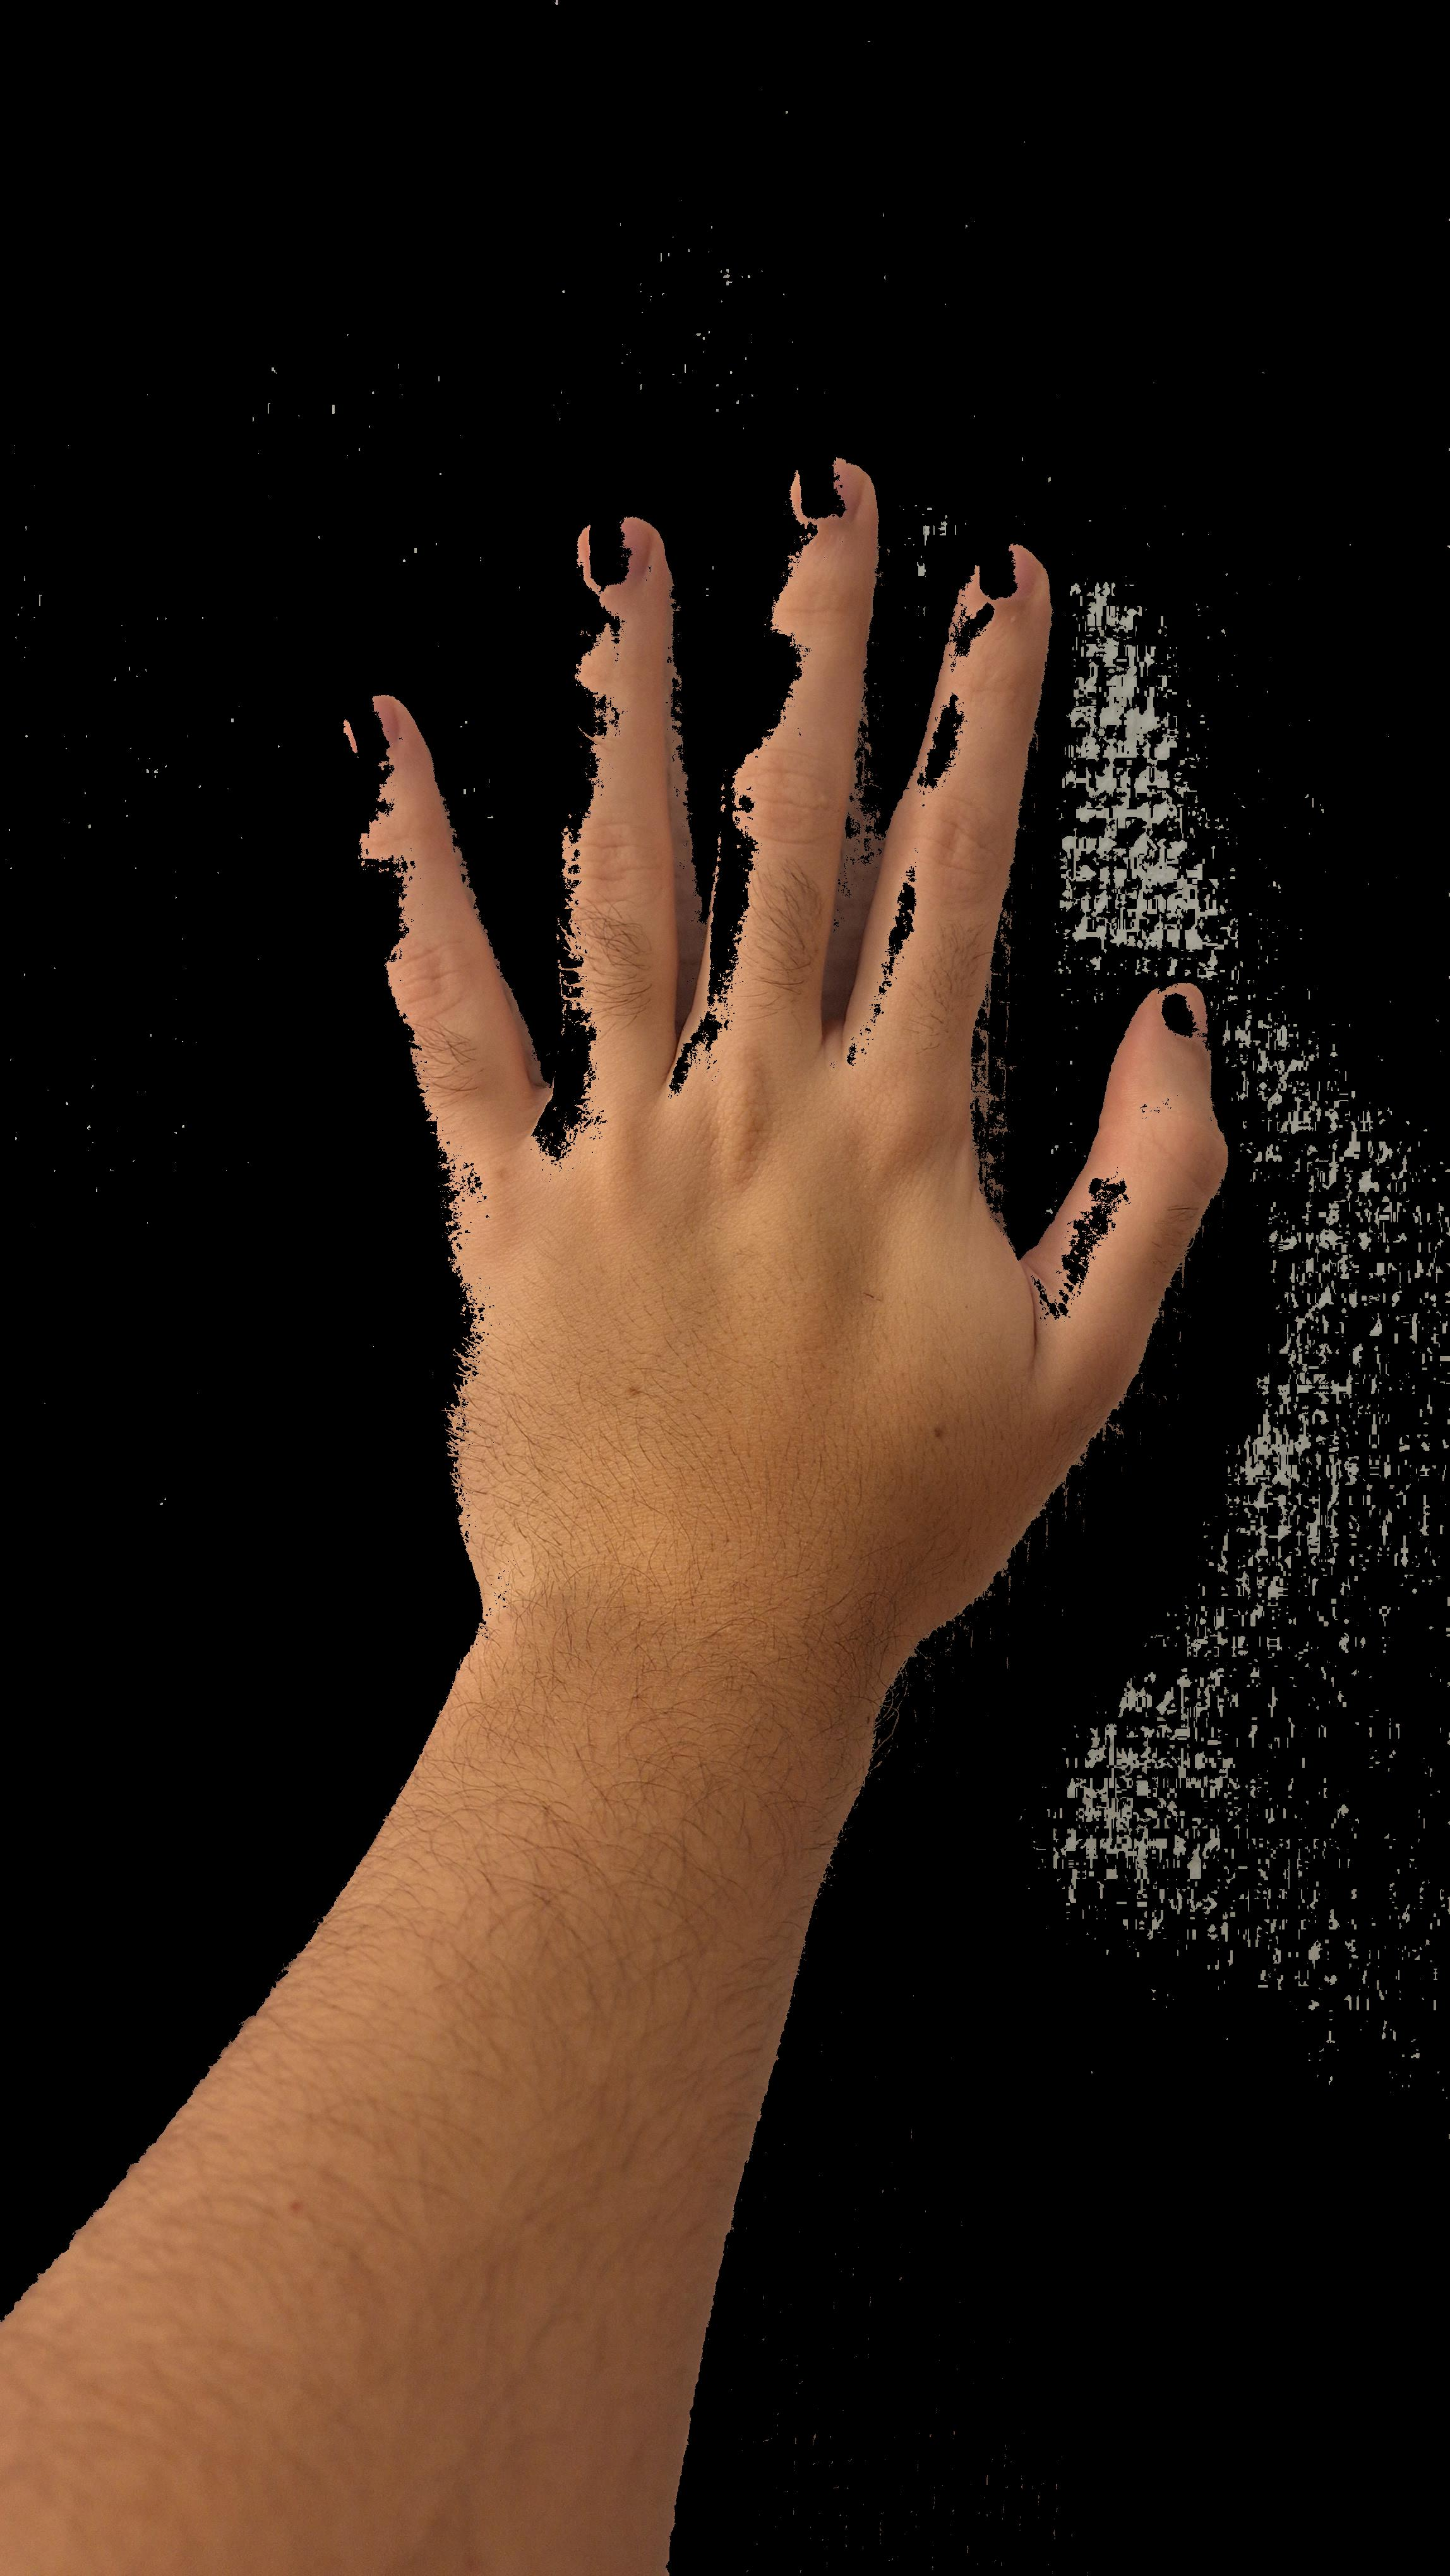
\includegraphics[width=0.3\linewidth]{../images/results/hand3_skin_hsv.jpg} & 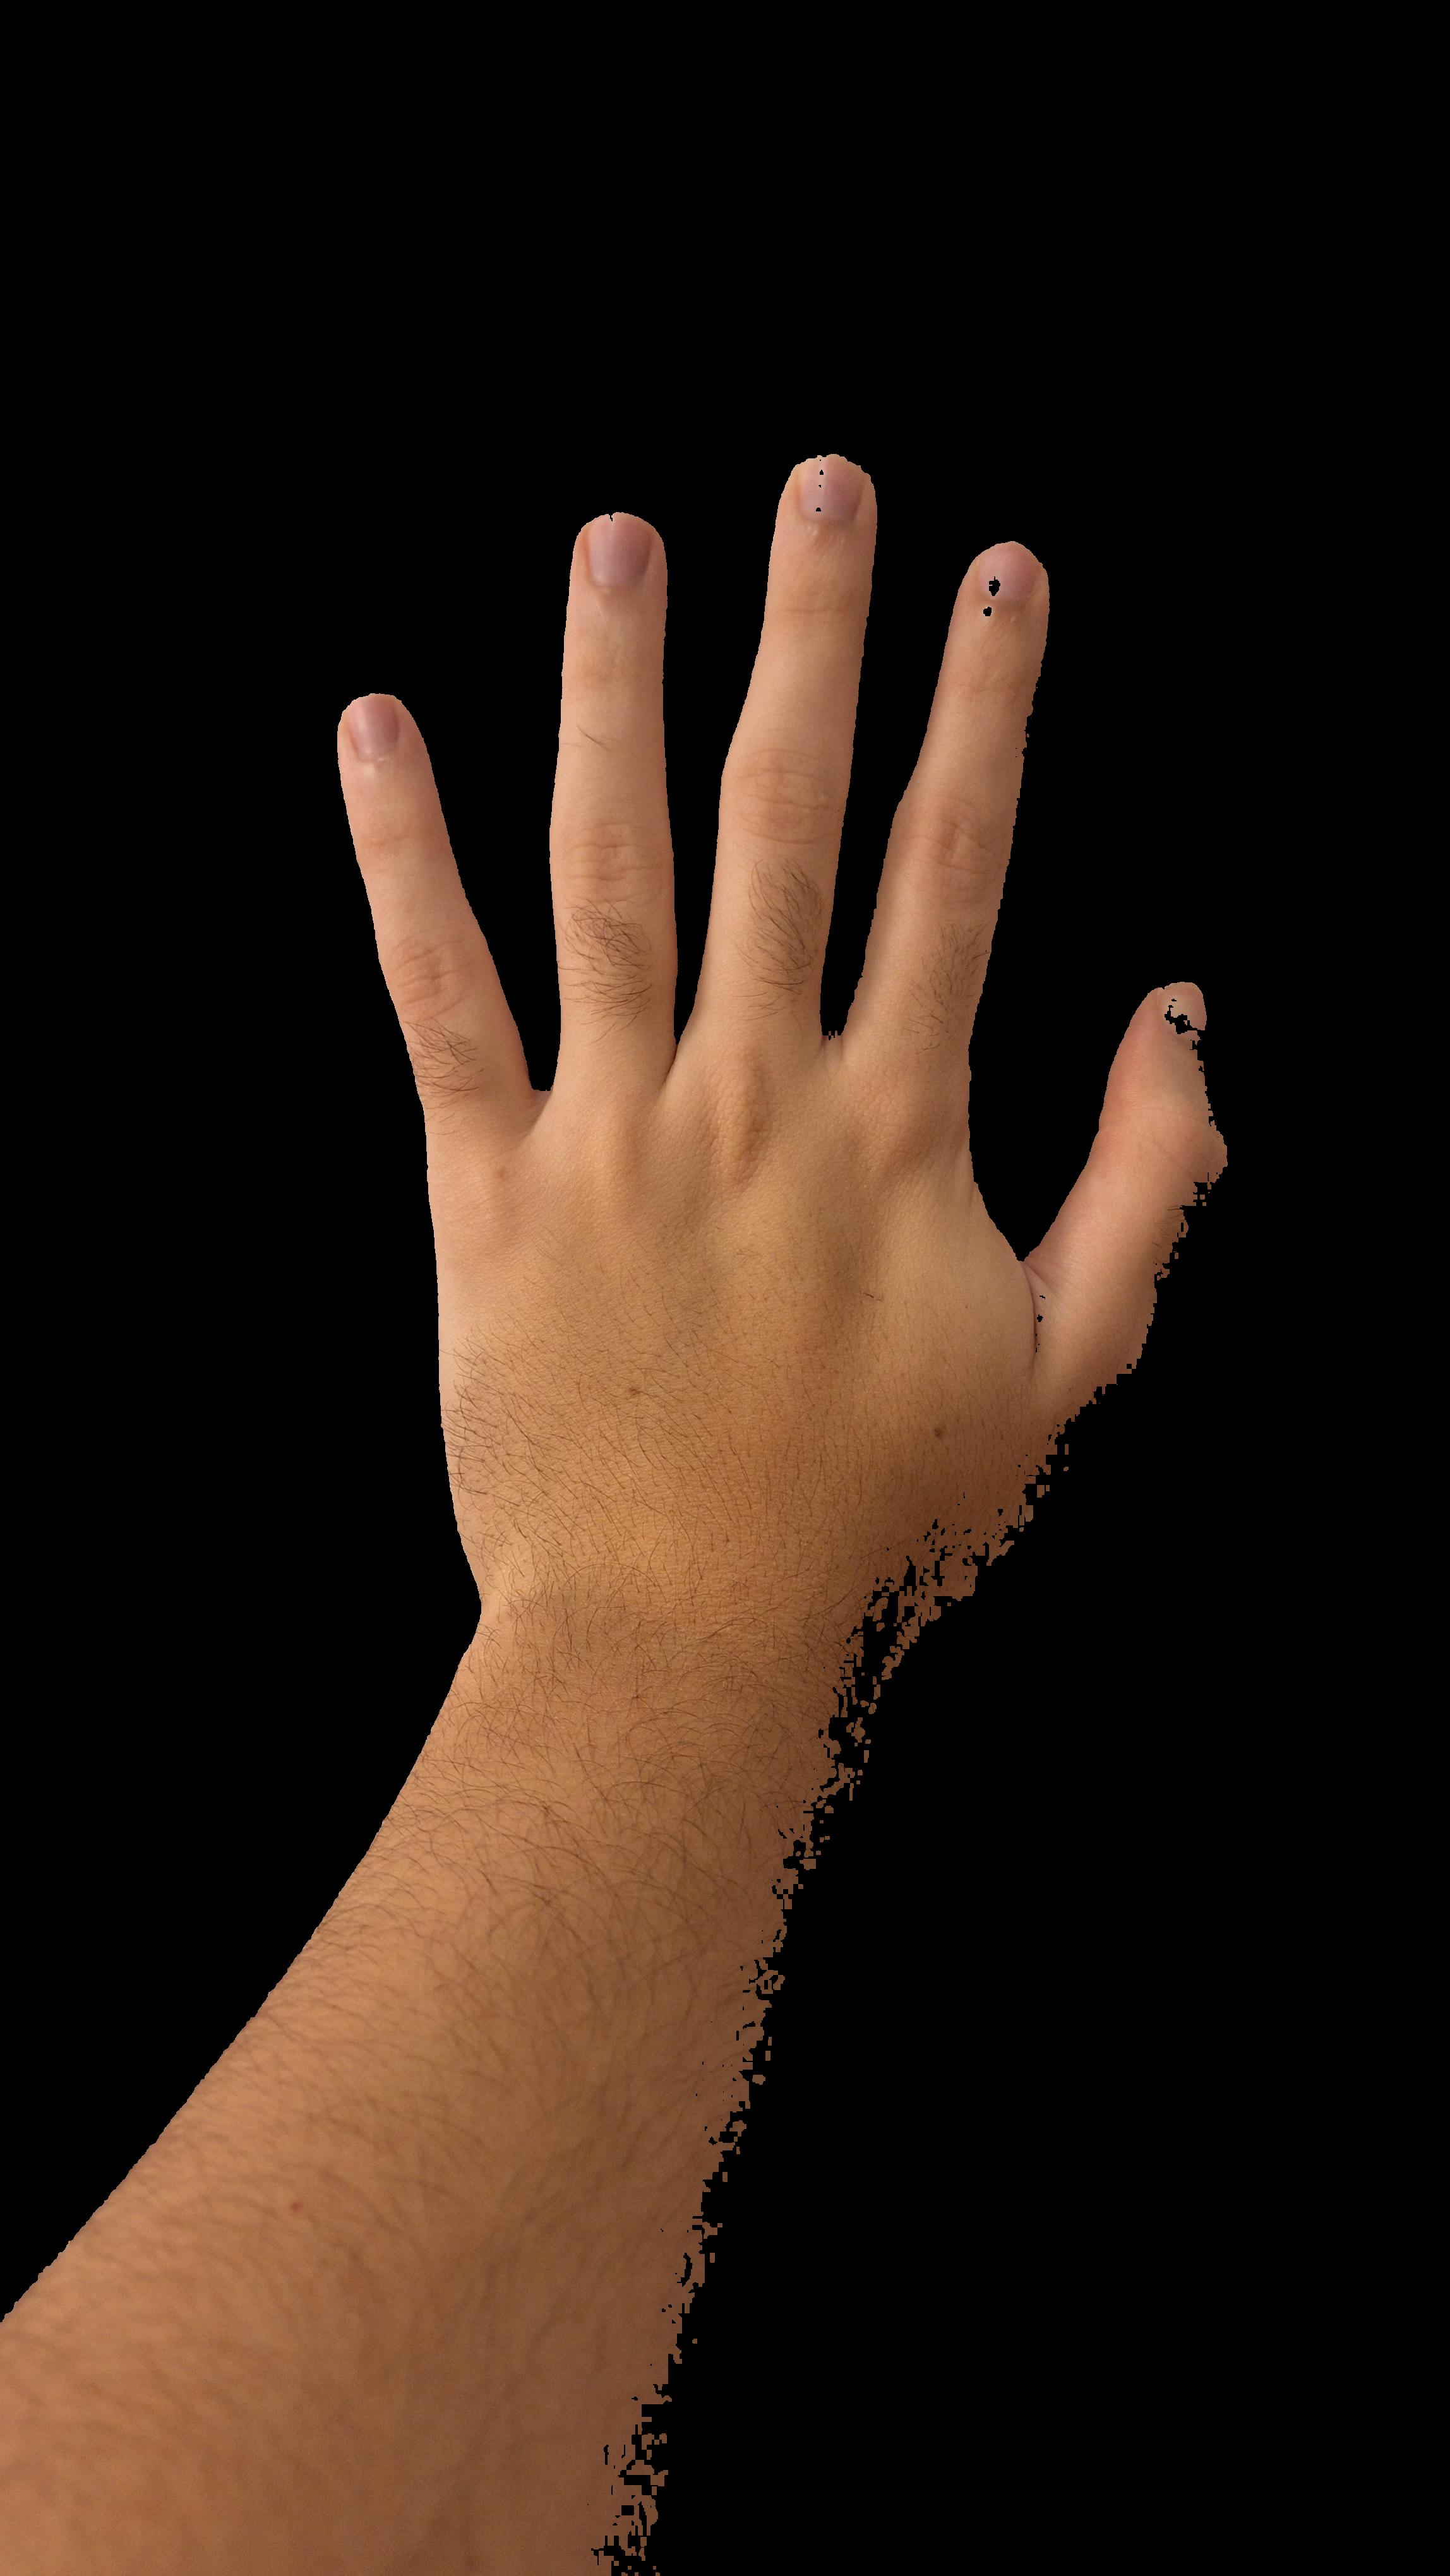
\includegraphics[width=0.3\linewidth]{../images/results/hand3_skin_ycc.jpg} \\
\end{tabular}
\caption{Image 3 results (HSV and YCbCr).}
\label{tab:images3}
\end{table}

\subsection{Precision}

The precision of our results was measured by comparing the results of our program with the ground truth images. We used the following formula to calculate the precision:

\begin{equation}
    Precision = \frac{TP}{TP + FP}
\end{equation}

Where TP is the number of true positives, and FP is the number of false positives.

\begin{table}[!htbp]
    \centering
    \begin{tabular}{|c|c|c|}
        \hline
        \textbf{Image} & \textbf{HSV Precision} & \textbf{YCbCr Precision} \\
        \hline
        1 & 90.7\% & 96\% \\
        \hline
        2 & 19.9\% & 100\% \\
        \hline
        3 & 93.7\% & 97.6\% \\
        \hline
    \end{tabular}
    \caption{Precision values for the three images in HSV and YCbCr color spaces.}
    \label{tab:precision}
\end{table}

\section{Conclusion}
 
This lab was crucial for the understanding of how lighting and color spaces can impact the efficacy of a segmentation.
The results between Image 1 and Image 2 bring about the best visualiation of how crucial lighting is for a photo, when changing the color spaces from HSV to YCbCr the results improved largely, yet for Image 2 the results were still somewhat underwhelming.
The background also plays a big role on the outcome of our program, in some cases the color of the wall, mixed with a certain lighting, were had to segment out.

In retorospect, when taking all of these factors into account, each use case is unique, therefore we need to fine tune the program and its parameters, like the mask range and color scheme,  for maximum efficiency.
Our results were satisfying but more tests can be conducted with better backgrounds and different lighting colors and intensities to further test the efficacy of our program.

% References
\bibliographystyle{IEEEtran}
% \bibliography{references}

\end{document}
